\section{Requisitos específicos}
\label{sec:req_esp}
\subsection{Interfaces externos}
\subsection{Requisitos funcionales}
\subsubsection{Gestión de usuarios}%USUARIOS
\begin{figure}[H]
    \centering
    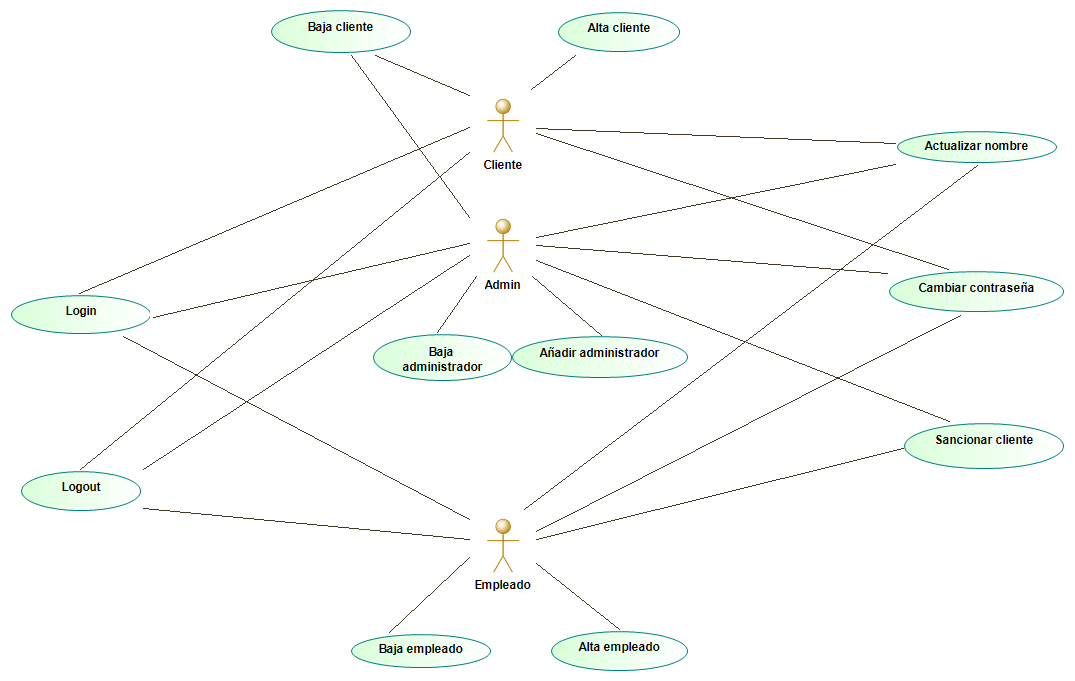
\includegraphics[width = 0.8\textwidth]{Use_Cases/Gestion_Usuarios.png}
\end{figure}
\paragraph{Alta cliente}
El usuario introduce su nombre usuario y contraseñas deseados en el sistema. Tras introducir los datos el sistema determina si ya existe dicho usuario. Si el nombre de usuario ya existe en la \gls{bd}, se informa de que dicho nombre no es valido. Si el nombre de usuario no se encuentra en la \gls{bd}, se procede a guardar los datos en la \gls{bd} y se informará al usuario del éxito de la operación.
\begin{figure}[H]
    \centering
    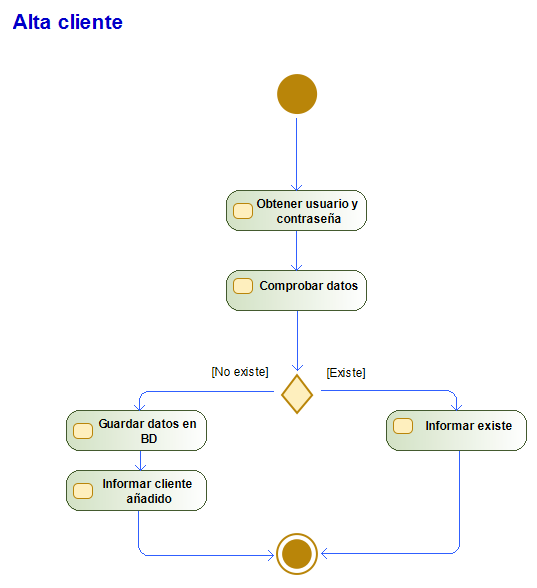
\includegraphics[width=0.8\textwidth]{Use_Cases/alta_cliente.png}
\end{figure}
\paragraph{Baja cliente}
El usuario solicita al sistema su baja, el administrador comprueba en la \gls{bd} si el usuario existe. En caso de ser encontrado, se borrarán sus datos de la \gls{bd}. En caso contrario, se informará al usuario de que no ha sido encontrado en la \gls{bd}
\begin{figure}[H]
    \centering
    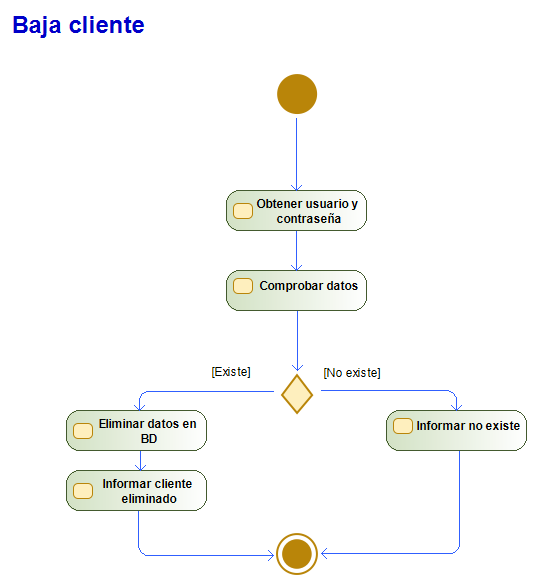
\includegraphics[width=0.8\textwidth]{Use_Cases/baja_cliente.png}
\end{figure}
\paragraph{Añadir Administrador}
Se solicita el usuario sus datos, un nombre de usuario y una contraseña. Si los datos coinciden se procede a buscar los datos del administrador en la \gls{bd}. En caso contrario, se informa de que los datos aportados no son válidos. Al buscar en la \gls{bd}, si el usuario no existe, se creará y se le darán permisos de administrador. En caso de ya existir, se avisará de ello.
\begin{figure}[H]
    \centering
    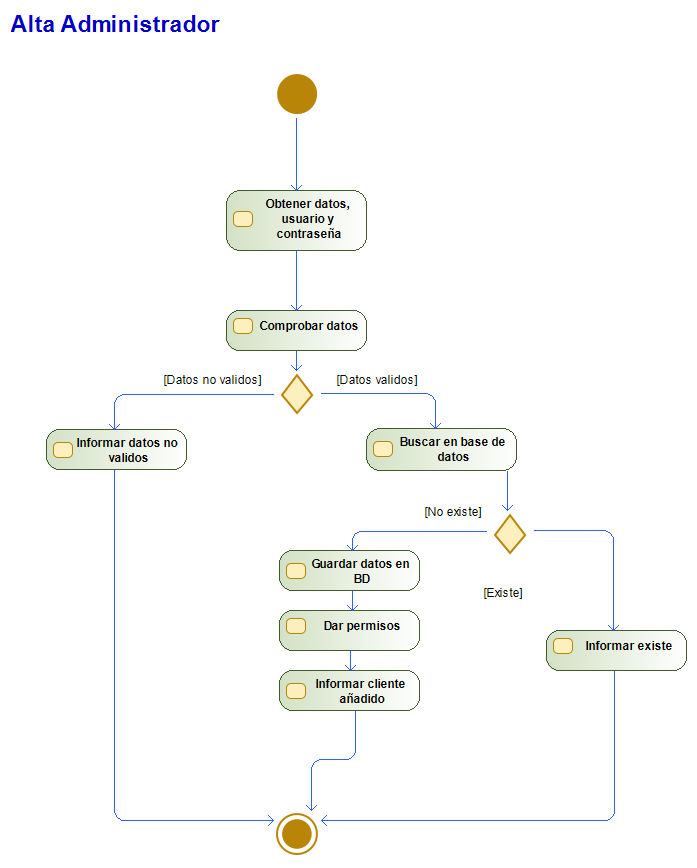
\includegraphics[width=0.8\textwidth]{Use_Cases/alta_admin.png}
\end{figure}
\paragraph{Baja administrador}
Se obtienen los datos del administrador y se buscan en la \gls{bd}. Si se encuentran se le quitarán permisos y se borrará el usuario, al terminar se informará del éxito de la operación. Por el contrario, si no se encuentra el usuario, se informa  de que se ha producido un error.
\begin{figure}[H]
    \centering
    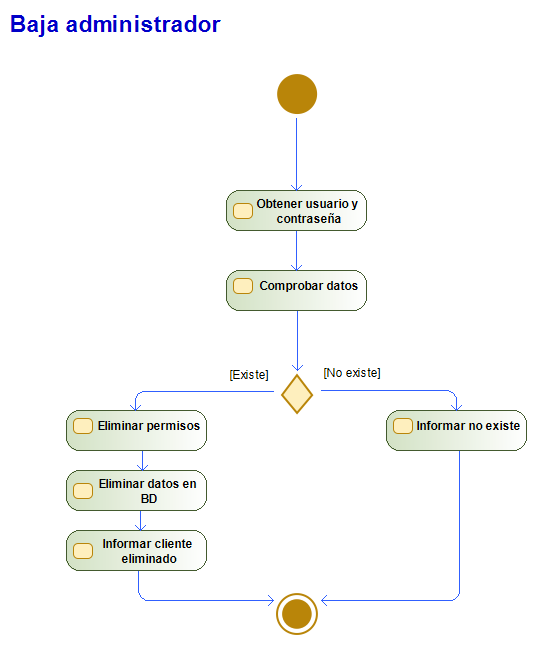
\includegraphics[width=0.8\textwidth]{Use_Cases/baja_admin.png}
\end{figure}
\paragraph{Alta empleado}
Se obtienen los datos del empleado y se buscan en la \gls{bd}. Si no se encuentra el empleado se crea el nuevo usuario y se informa de que ha tenido éxito, si se encuentra ya el usuario registrado se informara con un error.
\begin{figure}[H]
    \centering
    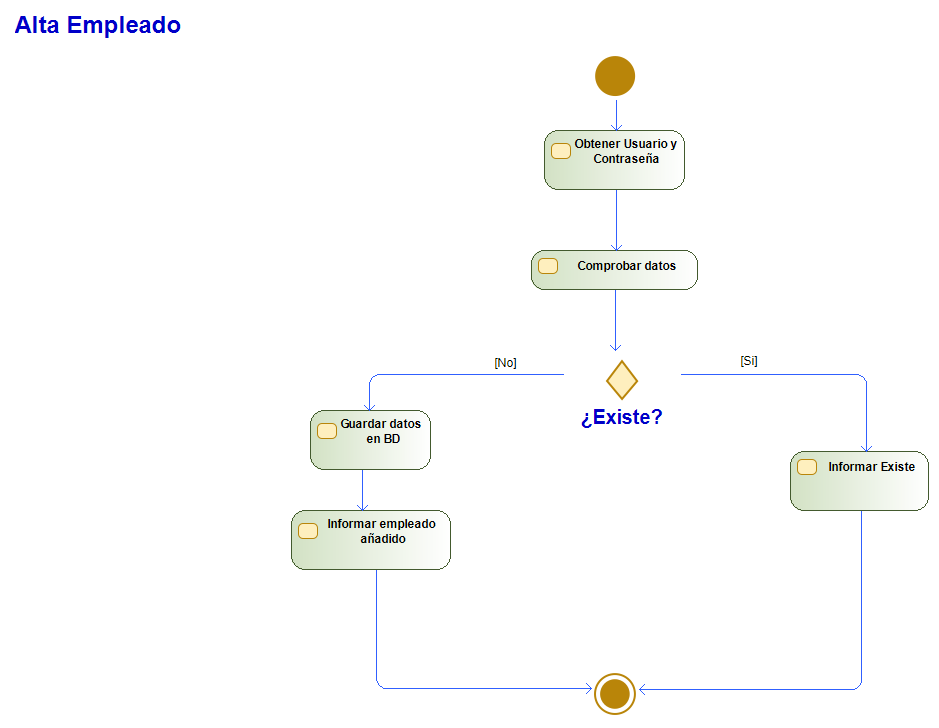
\includegraphics[width=0.8\textwidth]{Use_Cases/Alta_empleado.png}
\end{figure}
\paragraph{Baja empleado}
Se obtienen los datos del empleado y se buscan en la \gls{bd}. Si se encuentra se borrara el usuario y se informará de que la operación tuvo éxito, si el usuario no se encuentra se informará con un error
\begin{figure}[H]
    \centering
    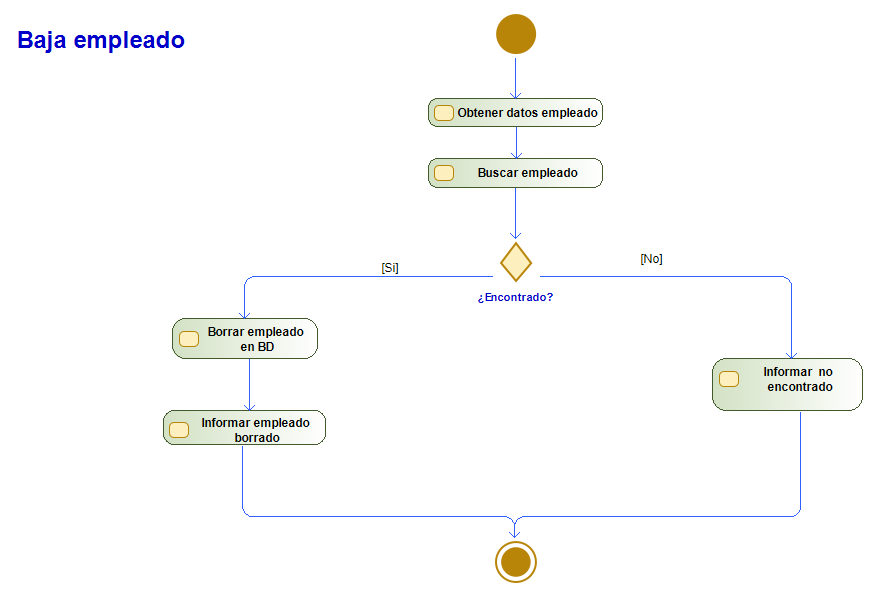
\includegraphics[width=0.8\textwidth]{Use_Cases/Baja empleado.png}
\end{figure}
\paragraph{Sancionar cliente}
Se comprueba si el aviso es una infracción de las normas, si es el cliente es un infractor reincidente en la \gls{bd}, si lo es se incrementa la magnitud de la sanción, sino se actualiza en la \gls{bd} y se sanciona, por otro lado si no es una infracción no se hace nada.
\begin{figure}[H]
    \centering
    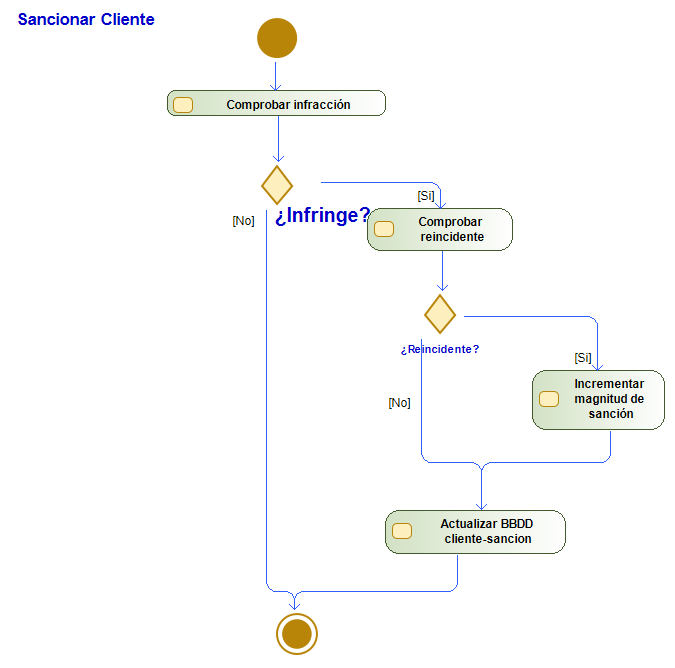
\includegraphics[width=0.8\textwidth]{Use_Cases/Sancionar Cliente.png}
\end{figure}
\paragraph{Cambiar nombre}
Se solicitan los datos del usuario y se comprueba en la \gls{bd} si existe o no, si existe se solicitan los datos a los que se quiere cambiar, después se comprueba si el nombre es válido, si lo es se actualizan los datos, sino se informa de que el nombre no es valido y se termina.
\begin{figure}[H]
    \centering
    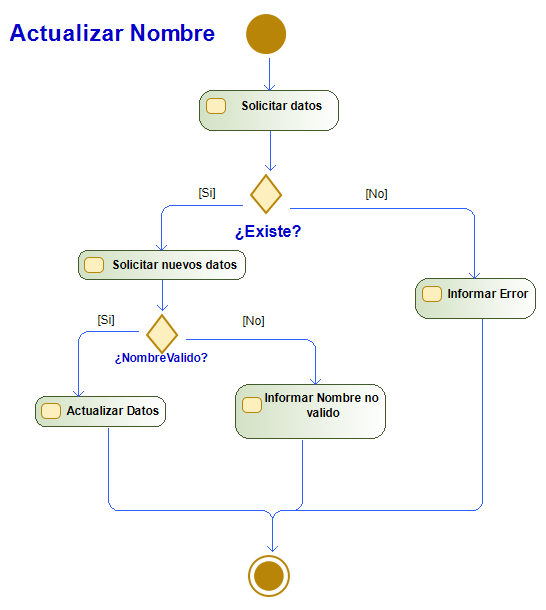
\includegraphics[width=0.8\textwidth]{Use_Cases/Actualizar Nombre.png}
\end{figure}
\paragraph{Cambiar contraseña}
El usuario indica su contraseña actual y el sistema comprueba si dicha contraseña es correcta o no. En caso de ser correcta el usuario indicará a continuación la nueva contraseña. Si esta contraseña es valida, el sistema indicará de que el cambio de contraseña ha sido satisfactorio.
\begin{figure}[H]
    \centering
    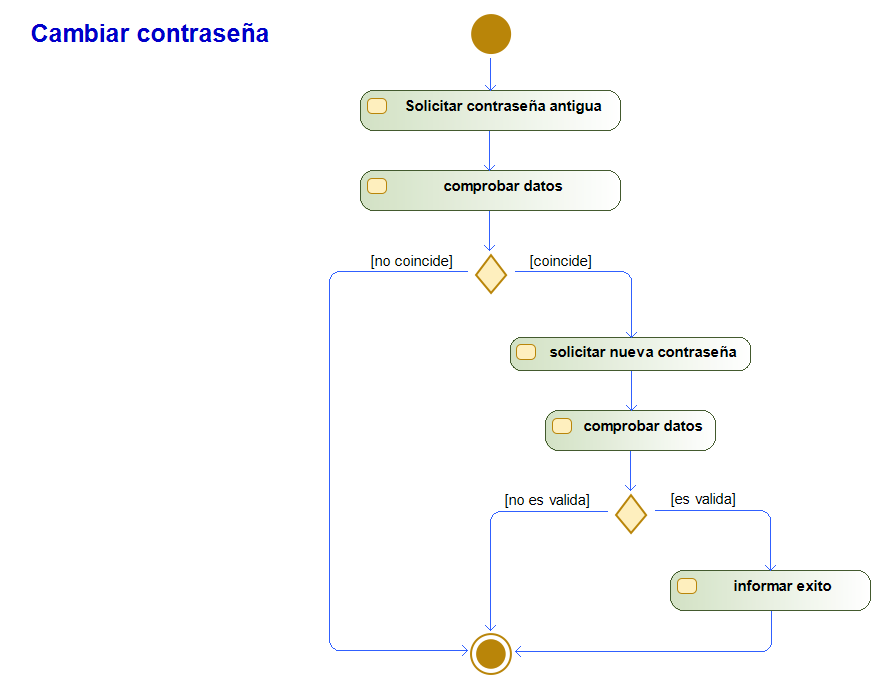
\includegraphics[width=0.8\textwidth]{Use_Cases/cambiar_contrasena.png}
\end{figure}
\paragraph{Login}
El usuario introduce su nombre usuario y contraseña en el sistema. Tras introducir los datos el sistema determina si son correctos o no. Si son correctos, el sistema indicará que el usuario se ha logueado correctamente. En caso contrario, se informa que no ha sido logueado.
\begin{figure}[H]
    \centering
    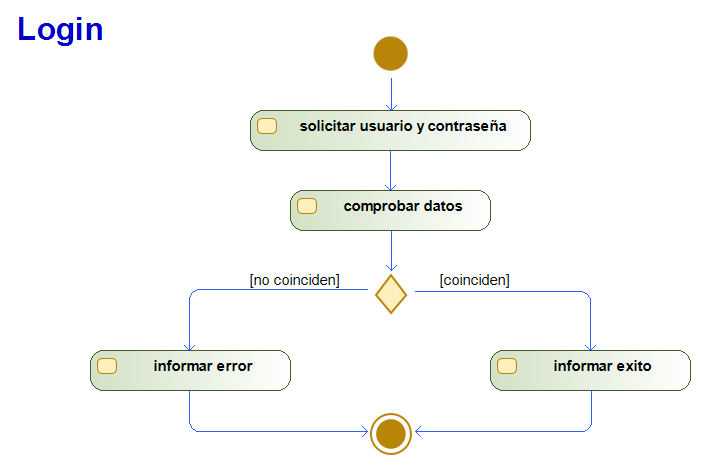
\includegraphics[width=0.8\textwidth]{Use_Cases/login.png}
\end{figure}
\paragraph{Logout}
EL usuario confirma que va a cerrar sesión. Si el usuario confirma que cierra sesión, el sistema indicará que se ha realizado la acción correctamente.
\begin{figure}[H]
    \centering
    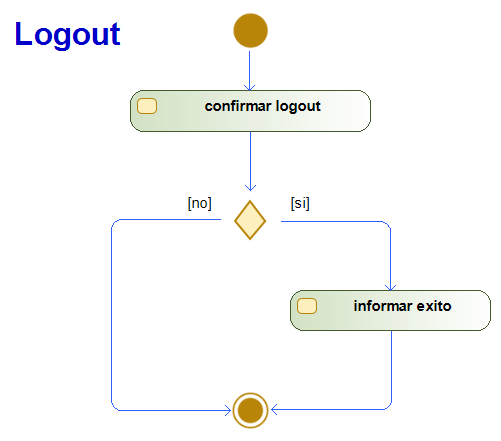
\includegraphics[width=0.8\textwidth]{Use_Cases/Logout.png}
\end{figure}
\subsubsection{Gestión de inventario}
\begin{figure}[H]
    \centering
    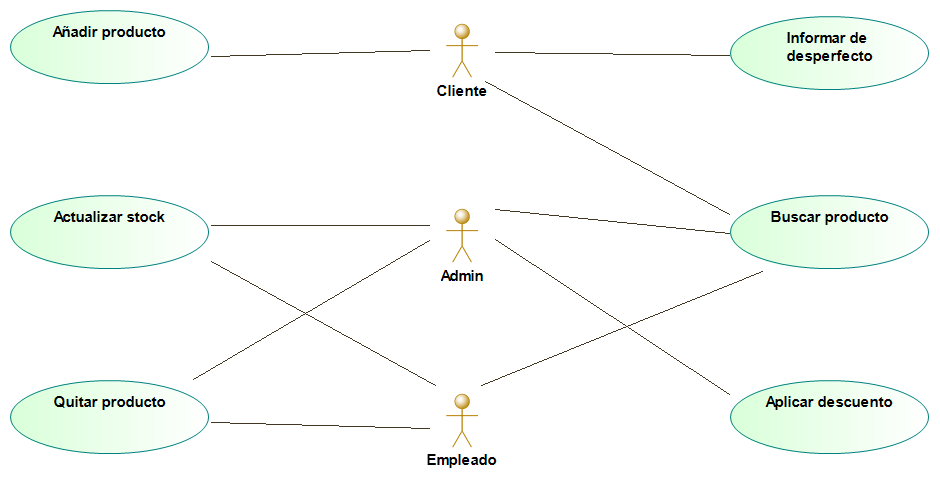
\includegraphics[width = 0.8\textwidth]{Use_Cases/gestion_de_inventario.png}
\end{figure}
\paragraph{Añadir producto}
\begin{figure}[H]
    \centering
    \includegraphics[width=0.8\textwidth]{Use_Cases/ProyectoIS_añadirProducto.png}
\end{figure}
\paragraph{Buscar producto}
\begin{figure}[H]
    \centering
    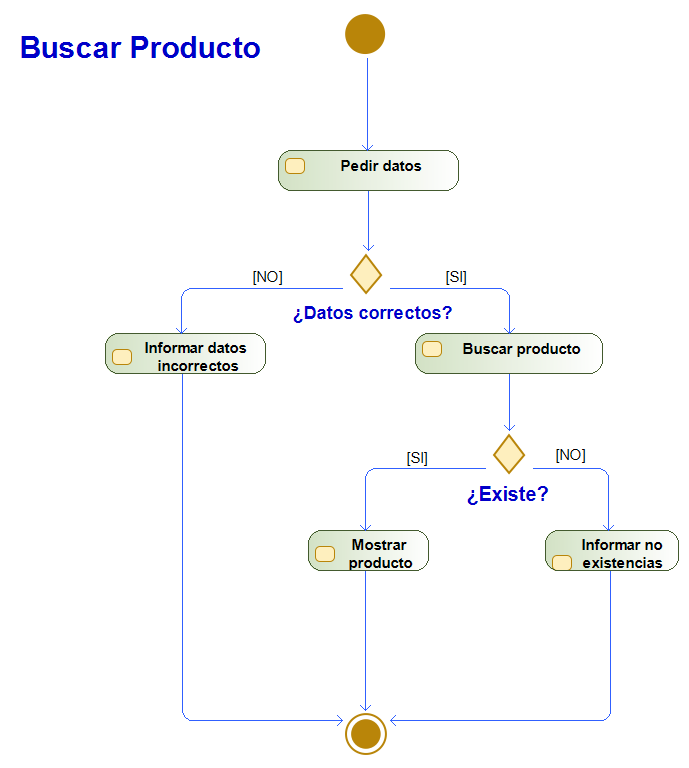
\includegraphics[width=0.8\textwidth]{Use_Cases/ProyectoIS_BuscarProducto.png}
\end{figure}
\paragraph{Actualizar stock}
\begin{figure}[H]
    \centering
    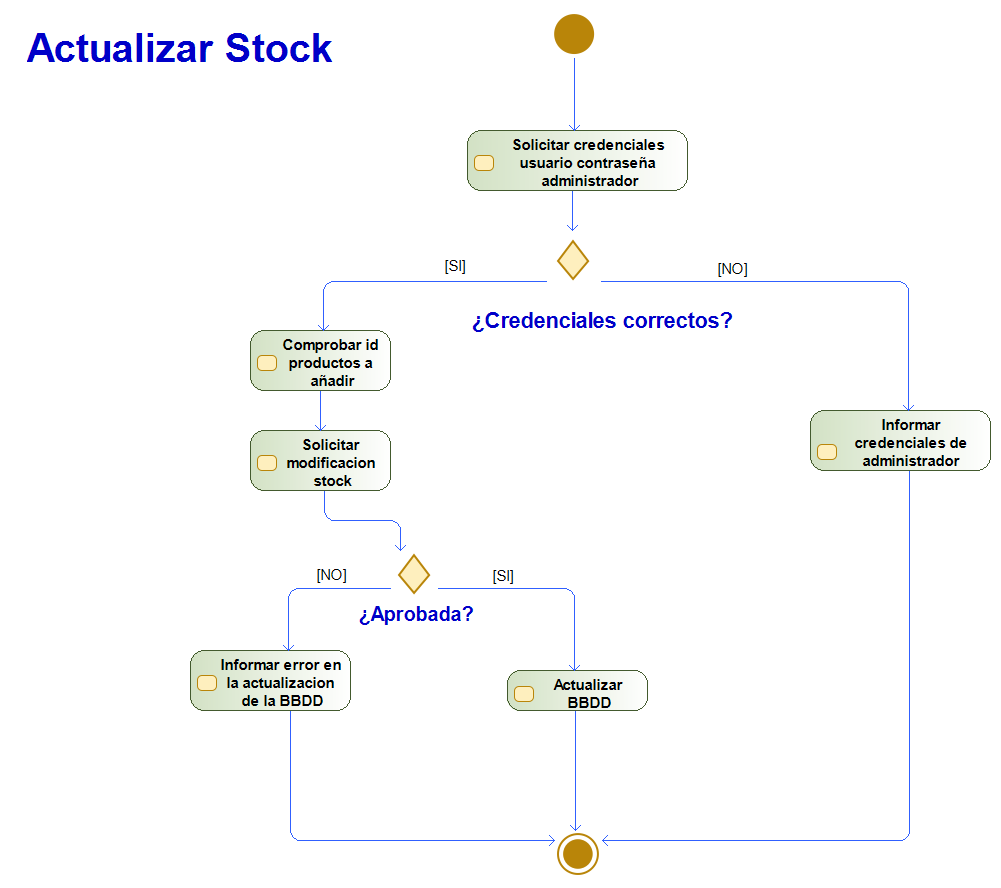
\includegraphics[width=0.8\textwidth]{Use_Cases/ProyectoIS_ActualizarStock.png}
\end{figure}
\paragraph{Quitar producto}
\begin{figure}[H]
    \centering
    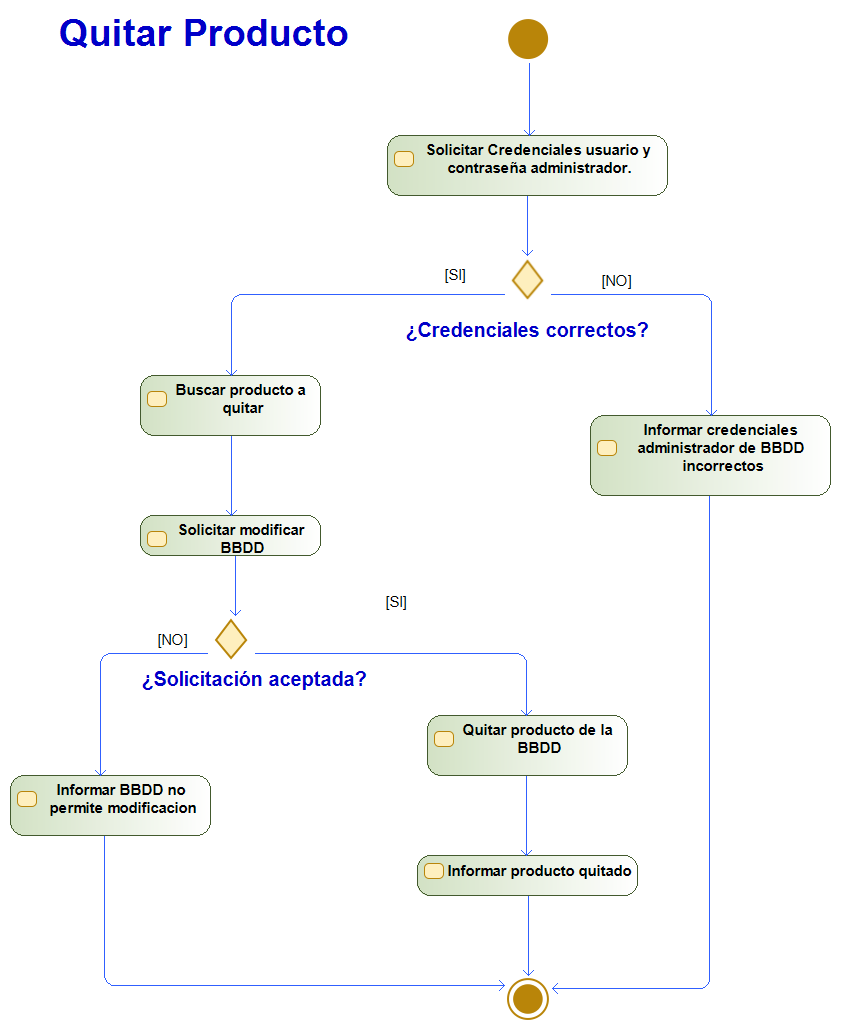
\includegraphics[width=0.8\textwidth]{Use_Cases/ProyectoIS_QuitarProducto.png}
\end{figure}
\paragraph{Aplicar descuento}
Ingresar usuario y contraseña, comprobar si la persona está registrada en la \gls{bd}. Si el usuario no existe sale. Si el usuario existe, selecciona la opción de descuentos, verifica si el cliente tiene derecho a un descuento, si el usuario no posee ninguna opción a descuenta sale, y si tiene opción a descuento lo aplica al producto y actualiza el precio final del producto o compra total.
\begin{figure}[H]
    \centering
    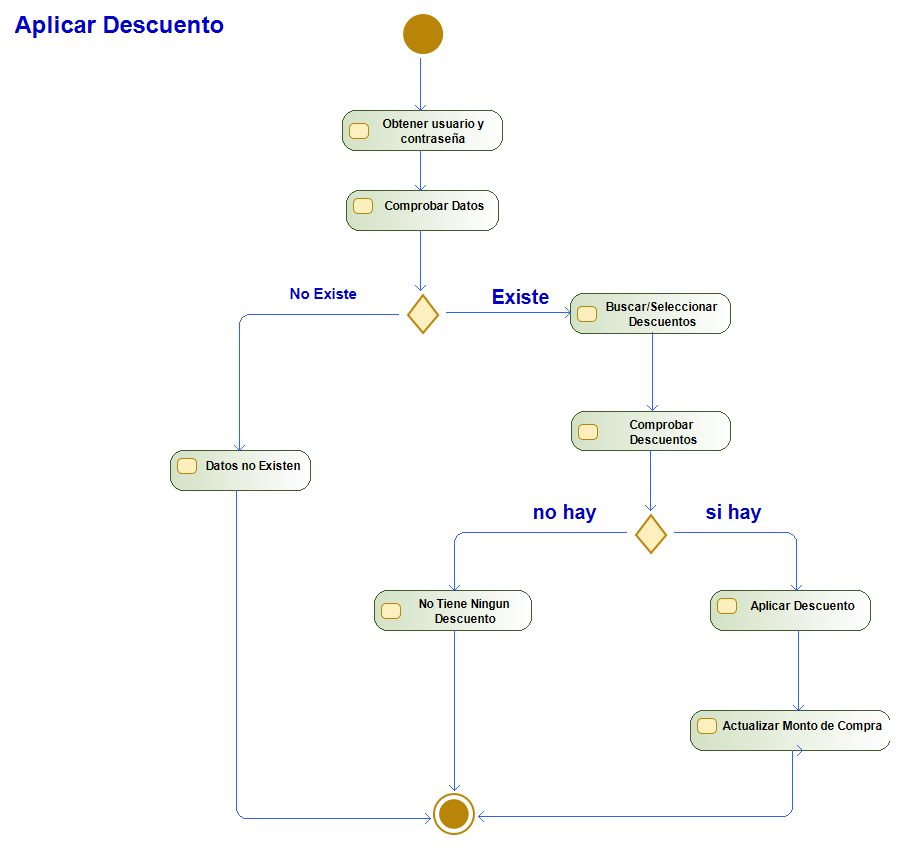
\includegraphics[width=0.8\textwidth]{Use_Cases/aplicar_descuento.png}
\end{figure}
\paragraph{Informar de desperfecto}
Ingresar usuario y contraseña, comprobar si la persona está registrada en la \gls{bd}. Si el usuario no existe sale. Si el usuario existe, selecciona un artículo, escribe el informe acerca de los desperfectos del mismo y al final lo envía.
\begin{figure}[H]
    \centering
    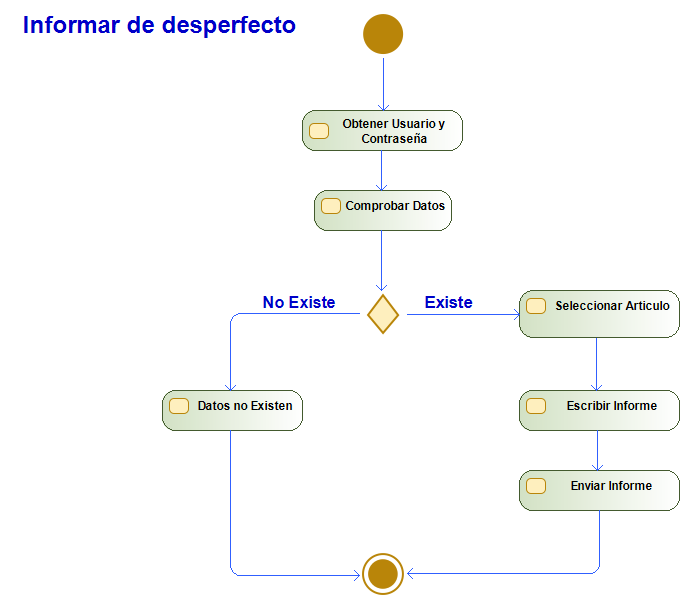
\includegraphics[width=0.8\textwidth]{Use_Cases/informar_de_desperfecto.png}
\end{figure}
\subsubsection{Gestión de pedidos}
Ingresar usuario y contraseña, comprobar si la persona está registrada en la \gls{bd}. Si el usuario no existe sale. Si el usuario existe, consulta en la \gls{bd} el listado de todos los pedidos realizados, selecciona mediante el número de pedido que desea consultar, verifica su estado ya sea en preparación, en tránsito o entregado.
\begin{figure}[H]
    \centering
    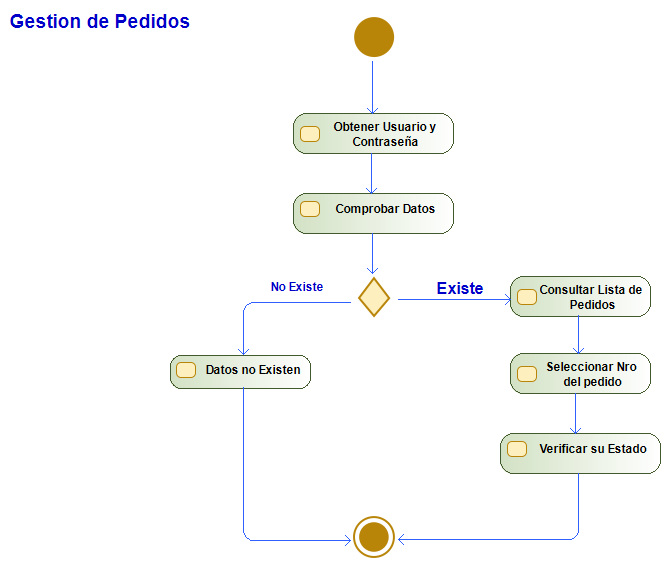
\includegraphics[width=0.8\textwidth]{Use_Cases/gestion_de_pedidos.png}
\end{figure}
\paragraph{Añadir promoción}
Ingresar usuario y contraseña, comprobar si la persona está registrada en la \gls{bd}. Si el usuario no existe sale. Si el usuario existe, consulta la lista de los productos en la \gls{bd}, se selecciona el producto(s) que se quiere promocionar, aplico la promoción, y actualizo el precio final del producto con la promoción incluida.
\begin{figure}[H]
    \centering
    \includegraphics[width=0.8\textwidth]{Use_Cases/añadir_promocion.png}
\end{figure}
\paragraph{Quitar promoción}
Se obtienen los datos del administrador y se comprueba si existe. Si existe, podrá consultar dicha promoción y eliminarla, al terminar se informará del éxito de la operación. Por el contrario si no se encuentra el usuario, se informará de que se ha producido un error.
\begin{figure}[H]
    \centering
    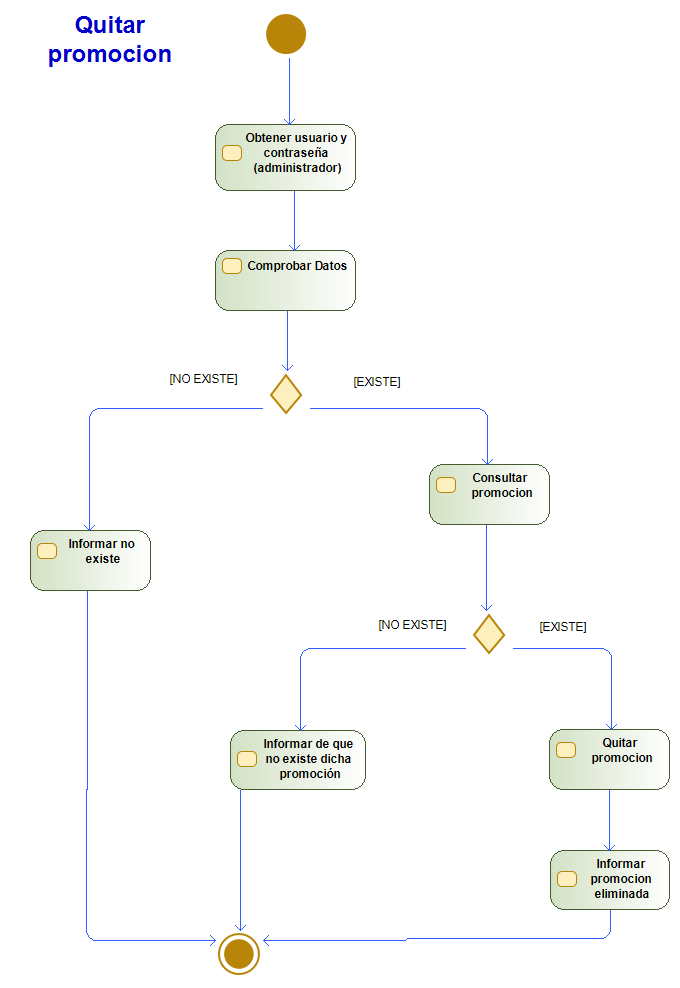
\includegraphics[width=0.8\textwidth]{Use_Cases/quitar_promocion.png}
\end{figure}
\paragraph{Compras}
Se introduce el nombre de usuario y la contraseña del cliente. Tras introducir los datos el sistema determina si son correctos o no. Si son correctos el usuario podrá añadir productos a su cesta y cuando quiera comprar alguno, se comprobará si tiene suficiente dinero en el monedero virtual, si lo tiene, se informará del éxito de su compra si no, se informará de saldo insuficiente. En el caso de no existir el usuario, se informará de ello.
\begin{figure}[H]
    \centering
    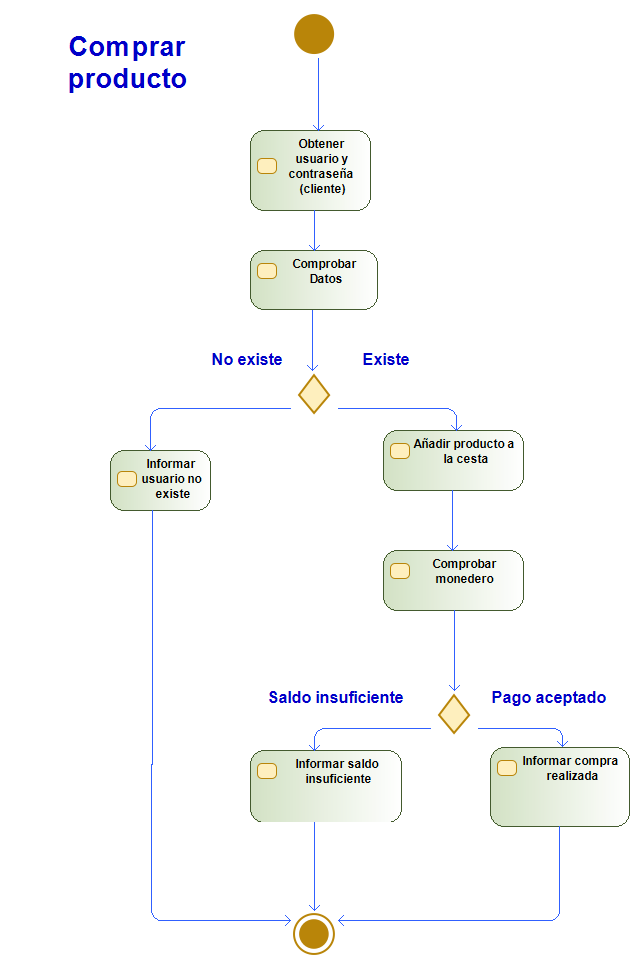
\includegraphics[width=0.8\textwidth]{Use_Cases/comprar_producto.png}
\end{figure}
\paragraph{Devolución de pedido}
Se introduce el usuario y la contraseña del cliente. Si existe, podrá consultar sus productos comprados y proceder a su devolución, en tal caso, el saldo de dicho producto comprado volverá al monedero virtual de dicho cliente. En caso de no existir dicho usuario, se informará de ello.
\begin{figure}[H]
    \centering
    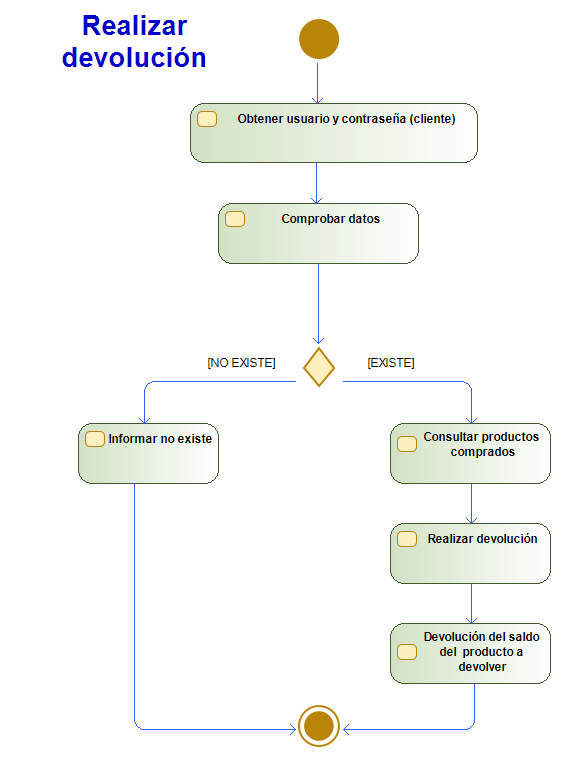
\includegraphics[width=0.8\textwidth]{Use_Cases/realizar_devolucion.png}
\end{figure}
\paragraph{Reservar producto}
Se obtiene el usuario y contraseña del usuario y se comprueban en la \gls{bd}. Si se encuentran, el cliente podrá consultar y reservar dicho producto en el caso de que tenga suficiente saldo en su monedero virtual, en tal caso se informará del éxito del producto reservado, si no, se informará al cliente de saldo insuficiente. En el caso de no existir usuario se informará de ello.
\begin{figure}[H]
    \centering
    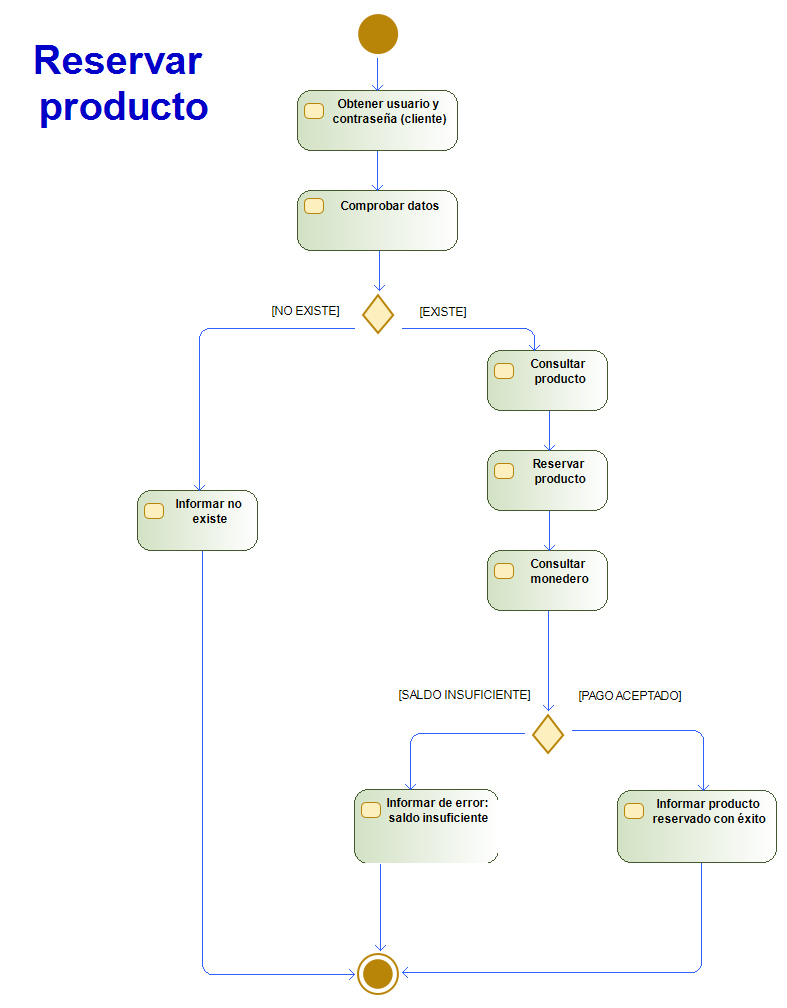
\includegraphics[width=0.8\textwidth]{Use_Cases/reservar_producto.png}
\end{figure}
\subsection{Requisitos de rendimiento}
Las operaciones de modificación de datos serán accesibles desde un mismo sitio físico, aunque en distintas máquinas, por ello la base de datos solo debe ser modificable desde un \gls{host} local. Los datos serán accesibles para lectura desde internet.
\subsection{Requisitos sobre la persistencia de datos}
\noindent\begin{tabularx}{\textwidth}{ l X }
    % \hline
    Producto-Cliente               & ``Un cliente no podrá comprar productos mientras esté sancionado"                                                \\
    Empleado-Producto              & ``El Empleado podrá dar de alta productos"                                                                       \\
    Empleado-Producto              & ``El Empleado podrá dar de baja productos"                                                                       \\
    Empleado-Producto              & ``El Empleado podrá modificar los datos de los juegos"                                                           \\
    Administrador-Producto-Cliente & ``El administrador podrá sancionar al cliente en caso de devolución fraudulenta del producto"                    \\
    Administrador-Empleado-Cliente & ``El administrador podrá cambiar las credenciales de los clientes y empleados bajo la demanda de dicho usuario'' \\
\end{tabularx}
\subsection{Restricciones de diseño}
El servidor sólo estaría disponible para ordenadores con Windows y Linux dado que este no cuenta con soporte para dispositivos Android ni dispositivos de la marca Apple.
\subsection{Atributos del sistema software}
La aplicación será software libre. Presentará una alta mantenibilidad sin perder fiabilidad para permitir que, en un futuro, más gente pueda contribuir al proyecto de manera sencilla y menos problemática.
